\documentclass[letterpaper,12pt,
				parkskip = half]{article}
\usepackage{tabularx} % extra features for tabular environment
\usepackage{amsmath}  % improve math presentation
\usepackage{graphicx} % takes care of graphic including machinery
\usepackage[margin=1in,letterpaper]{geometry} % decreases margins
\usepackage{cite} % takes care of citations
\usepackage[ngerman]{babel}
\usepackage[final]{hyperref} % adds hyper links inside the generated pdf file
\hypersetup{
	colorlinks=true,       % false: boxed links; true: colored links
	linkcolor=blue,        % color of internal links
	citecolor=blue,        % color of links to bibliography
	filecolor=magenta,     % color of file links
	urlcolor=blue         
}
\usepackage{blindtext}
\usepackage{wrapfig}
\usepackage{graphicx}
\usepackage{subcaption}
\usepackage{parskip}
\captionsetup{compatibility=false}
%++++++++++++++++++++++++++++++++++++++++


\begin{document}

\title{How To Erstell The Aufbauplan}
%\author{A. Partner, B. Partner, and C. Partner}
\date{\today}
\maketitle


\section{Einleitung}

Ein Aufbauplan eines Camps wird für die Versammlungsanmeldung benötigt. Änderungen Am Aufbauplan im Nachhinein sind am einfachsten, wenn der Plan digital erstellt wurde. In diesem Dokument wird die Erstellung eines Aufbauplans mit Inkscape\footnote{\texttt{https://inkscape.org}} erklärt. Inkscape ist kostenlos und open-source. Der Schritt \ref{kartenabschnitt} dieses How-To's ist auch nützlich, wenn eine andere Software als Inkscape verwendet wird.


%TODO WO
Ein beispielhafter Aufbauplan findet ihr hier:BLABLA. Dieser kann gerne als Vorlage verwendet werden!

\section{Einführung in Inkscape}

Inkscape ist ein Programm mit sehr vielen Funktionen, für die Erstellung des Aufbauplans wird nur ein Bruchteil benötigt. Die wichtigsten werden Funktionen werden im offiziellen Inkscape-Tutorial \footnote{\texttt{https://inkscape.org/doc/tutorials/basic/tutorial-basic.html}} erklärt. Außerdem gibt es einige ausführliche Videotutorials\footnote{\texttt{https://www.youtube.com/watch?v=zUIOEXssTSE}} (Beides auf Englisch).

\begin{wrapfigure}{r}{0.4\textwidth}
	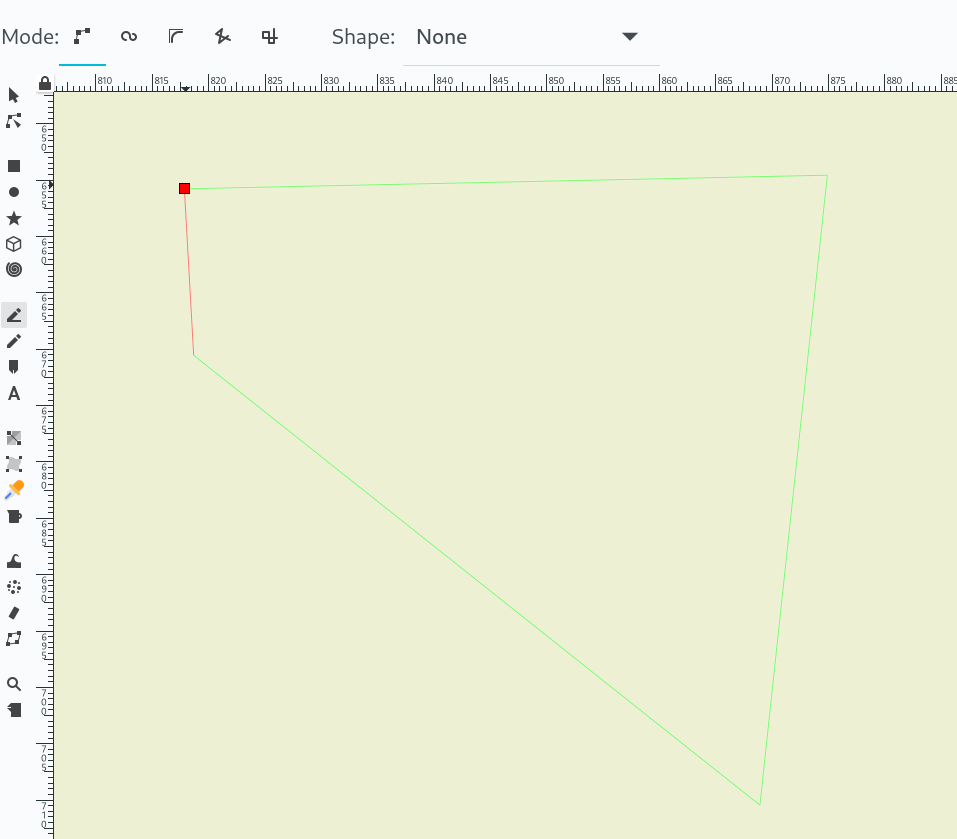
\includegraphics[width=0.3\textwidth]{Images/area.png}
	\caption{Zeichnen einer Fläche}
	\label{fig:area}
\end{wrapfigure}

Mit vielen Funktionen kann man sich am besten durchs Ausprobieren, z. B. an der Aufbauplanvorlage, vertraut machen.




\paragraph{Farben}
Um die Farbe eines Objektes zu verändern muss erst das Objekt angeklickt werden. Dann \texttt{Shift+Ctrl+F} drücken. Es öffnet sich die Farbübersicht.



\paragraph{Flächen}
Mit dem ersten Stift-Tool können Flächen gezeichnet werden, um z. B. die privaten Zeltflächen zu zeichnen. Dazu muss der letzte Punkt des gezeichneten Pfades auf den ersten Punkt geklickt werden.
\clearpage
\begin{wrapfigure}{r}{0.4\textwidth}
	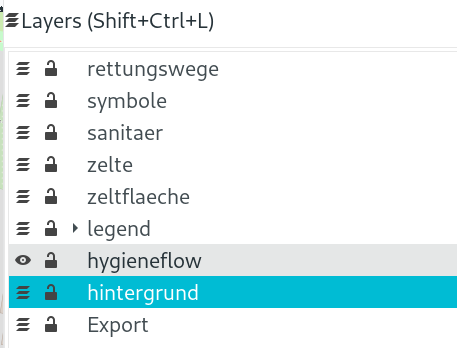
\includegraphics[width=0.3\textwidth]{Images/layers.png}
	\caption{Ebenen des Aufbauplans}
	\label{fig:layers}
\end{wrapfigure}


\paragraph{Ebenen}

Mit Inkscape können Objekte auf unterschiedlichen Ebenen (englisch: Layers) strukturiert. In Abbildung \ref{fig:layers} sind die unterschiedlichen Ebenen des Beispielaufbauplans dargestellt. Diese können mit \texttt{Shift+Ctrl+L} angezeigt werden. Mit einem Klick auf das Auge oder die drei Ebenen können die Ebenen ein- und ausgeblendet werden. Unter dem Menüpunkt \texttt{Layer > Move Selection to Layer...} können selektierte Objekte zwischen Ebenen hin und her geschoben werden. 


\paragraph{Ansaugfunktion}

Es gibt die Funktion, dass Objekte, wenn man sie bewegt, sich gegenseitig ansaugen, das ist manchmal super praktisch, manchmal aber auch super nervig.
Auf der rechten Toolbar ganz oben gibt es die Option \texttt{Enable Snapping}. Damit kann das Ansaugen an und aus geschaltet werden.

\section{Kartenausschnitt runterladen und einfügen}
\label{kartenabschnitt}

Als Hintergrund des Aufbauplans dient am besten ein Kartenausschnitt, z. B. von OpenStreetMap\footnote{\texttt{https://www.openstreetmap.org}}, welcher von dort exportiert wird.

\begin{figure}[!h]
%\begin{wrapfigure}{r}{0.5\textwidth}

	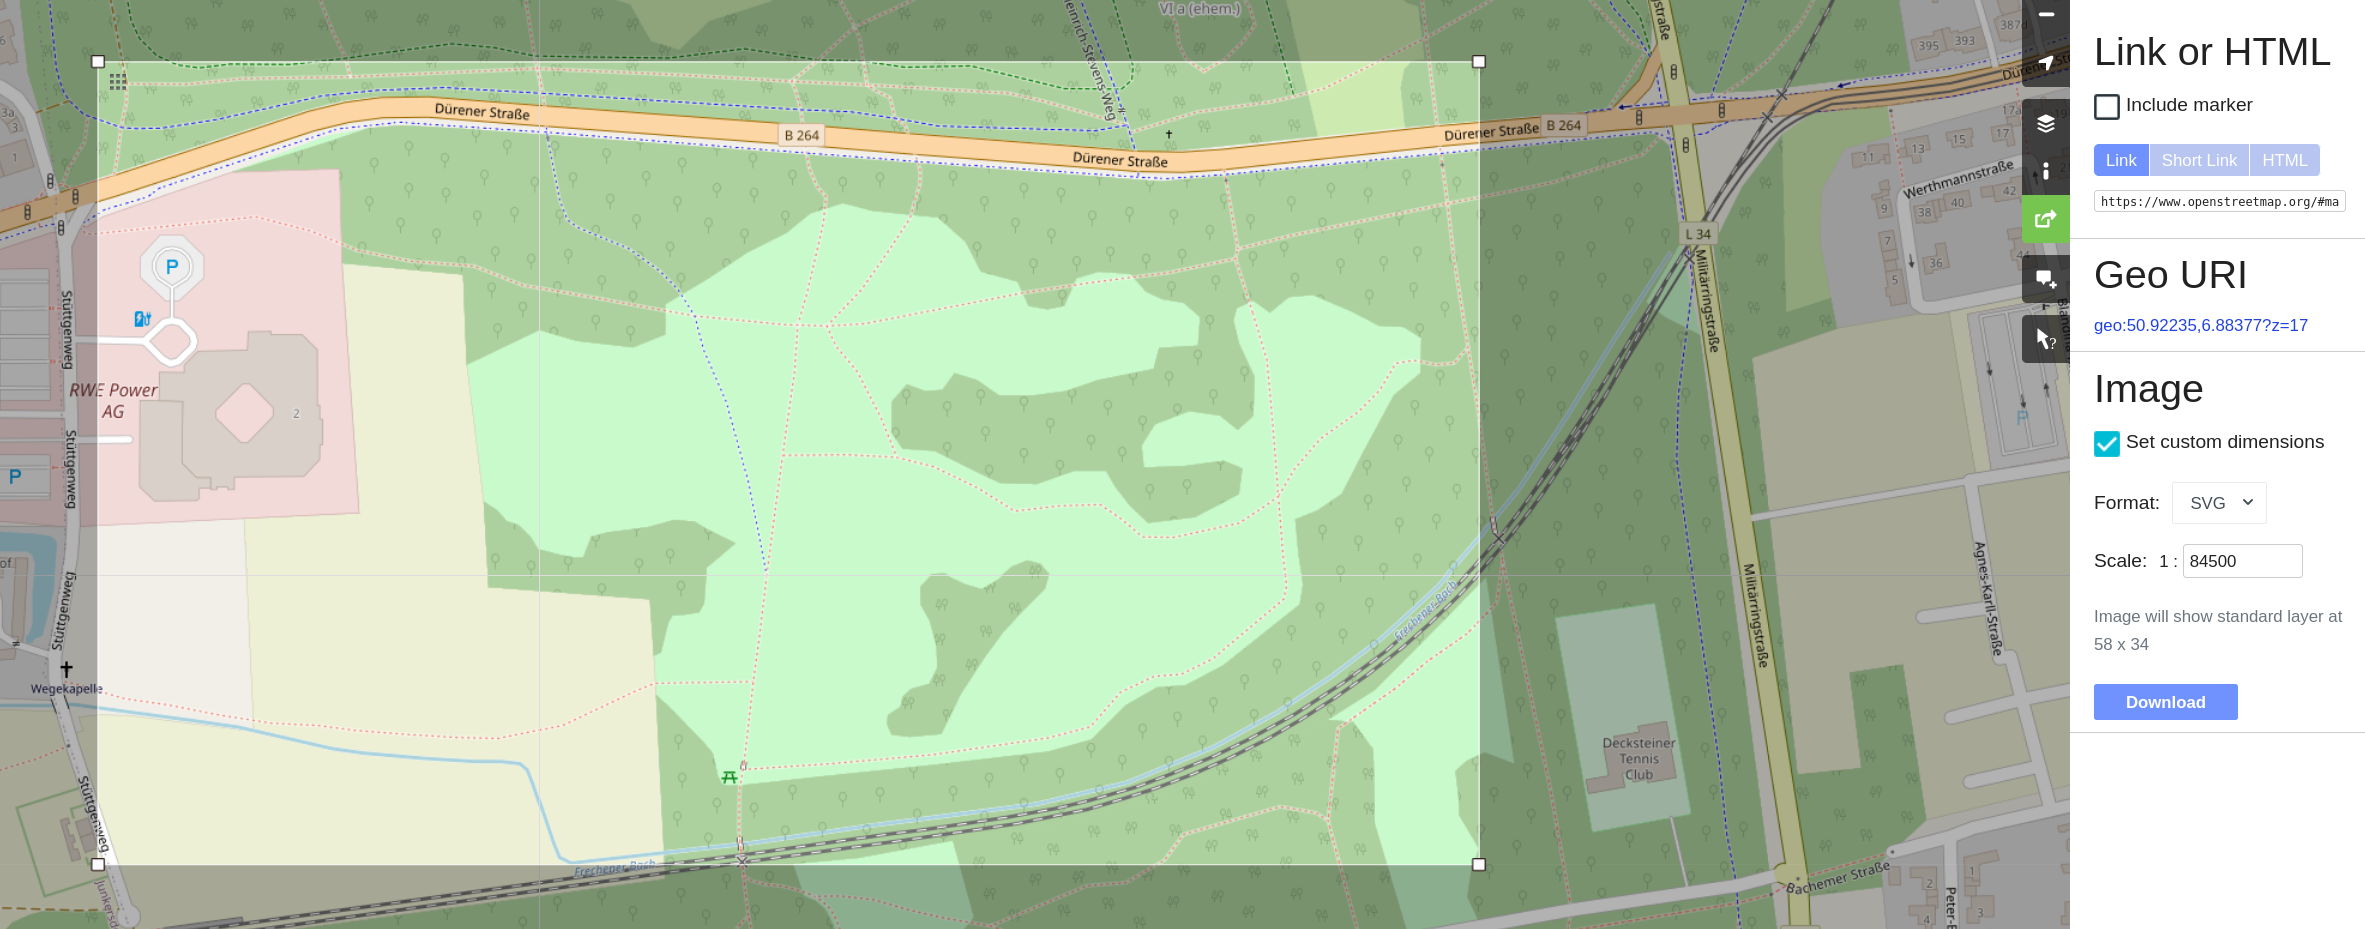
\includegraphics[width=\textwidth]{Images/exportosm.png}

	\caption{Kartenexport aus OpenStreetMap}

	\label{fig:exportosm}
\end{figure}
%\end{wrapfigure}

Dazu die Fläche ins Fenster nehmen, auf der das Camp sein wird. Am rechten Fensterrand auf das dritte Symbol von unten \flqq{}Share\frqq{} klicken. Unter \flqq{}Image\frqq{} \texttt{Set custom dimensions} anhaken. Jetzt kommt dieser Bereich, mit dem passgenau der Bereich bestimmt werden kann, der exportiert werden soll. Jetzt noch das Format \texttt{SVG} auswählen und \flqq{}Download\frqq{} drücken (siehe Abbildung \ref{fig:exportosm}). 
Mit einer \texttt{SVG}-Karte ist Inkscape manchmal etwas langsam, die Karte als \texttt{PNG} runterzuladen geht auch, ist aber verpixelt, wenn man nah ran zoomt. 

Jetzt kann die von OpenStreetMap exportierte Karte mit Inkscape geöffnet werden. Die Karte am besten gleich auf eine neue Ebene \flqq{}Hintergrund\frqq{} oder so verschieben.

Natürlich funktioniert auch ein Screenshot von einer Satellitenkarte, wird aber auch verpixelt wenn man ranzoomt!

\section{Karte richtig skalieren}

Um den Campplan maßstabsgetreu zu zeichnen ist es am besten die Karte zu Beginn zu skalieren. Durch eine skalierte Karte wird es auch viel einfacher die Zelt-, Infrastruktur- und Weggrößen richtig zu treffen.

Dazu ist es notwendig die Länge eines Objektes auf der Karte zu kennen, nach dem die restliche Karte skaliert werden kann.
Für das Beispiel in Abbildung \ref{fig:exportosm} wird die linke Gebäudeseite genommen. Diese kann mit dem Tool TIM-online\footnote{\texttt{https://www.tim-online.nrw.de/tim-online2/}} nachgemessen werden (s. Abbildung \ref{fig:tim}).

\begin{figure}[!h]
\centering
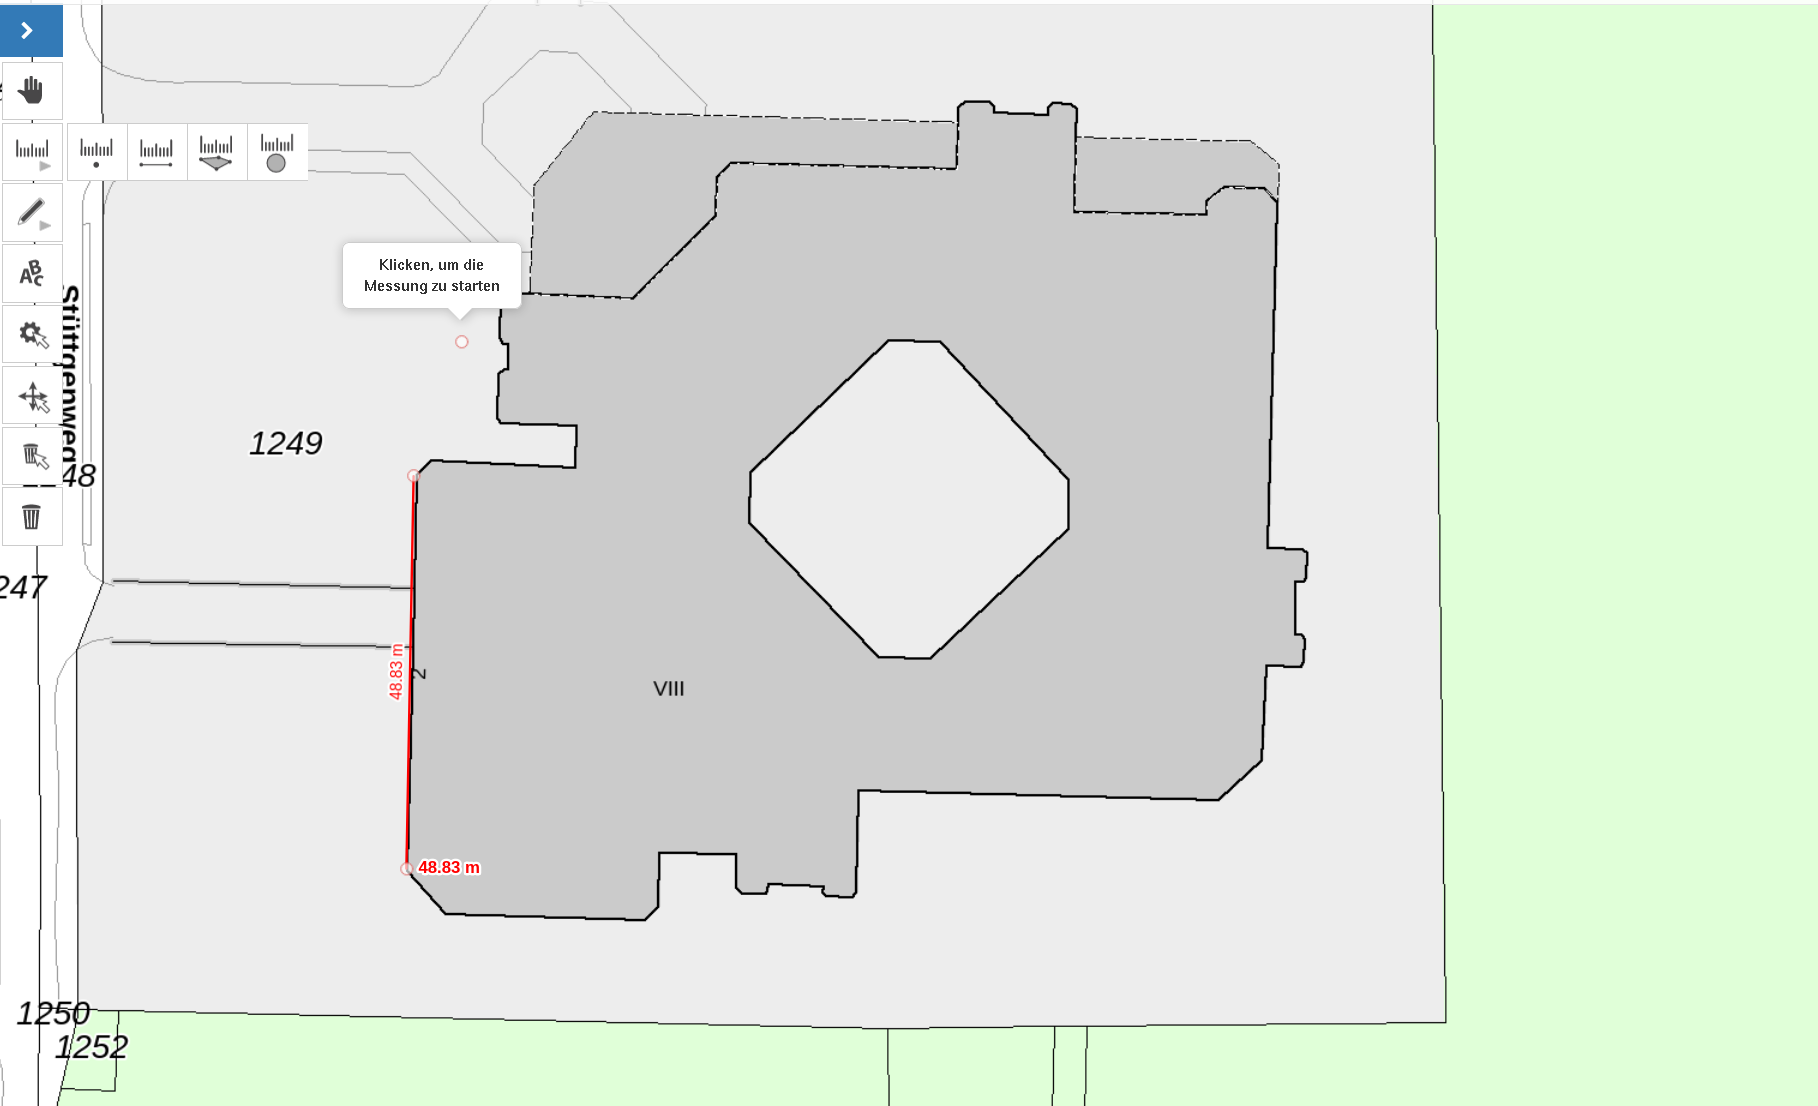
\includegraphics[width=0.8\textwidth]{Images/timonline.png}
\caption{Entfernung messen mit TIM-online}
\label{fig:tim}
\end{figure}

Ein Meter in der Karte soll auf einen Millimeter in Inkscape skaliert werden. Dazu gibt es eine Inkscape Extension \flqq{}RealScale\frqq{}\footnote{\texttt{https://inkscape.org/\~{}Moini/\%E2\%98\%85realscale-resize-by-line-of-known-length}}. Unter dem Link in der Fußnote ist die Installation erklärt, die aktuelle Version kann hier: \\ \texttt{https://gitlab.com/Moini/inkscape-realscale-exten}\\ \texttt{sion/-/repository/archive.zip?ref=master} runtergeladen werden.

Zum Skalieren Inkscape einmal neustarten. An der ausgemessenen Kante eine Linie mit dem Stift-Tool ziehen. Die gezogene Linie auswählen. Jetzt \texttt{Shift} halten und die Karte anklicken. Auf \texttt{Extensions > Scaling > RealScale...} gehen. 

Für \flqq{}Length of scaling path\frqq{} die in TIM-online gemessene Länge der Hausseite in Metern eingeben.
Den Rest wie in Abbildung \ref{fig:scaling_ausfuellen}. und \flqq{}Apply\frqq{} drücken.

\begin{figure}[!h]
%	\begin{subfigure}{0.5\textwidth}
		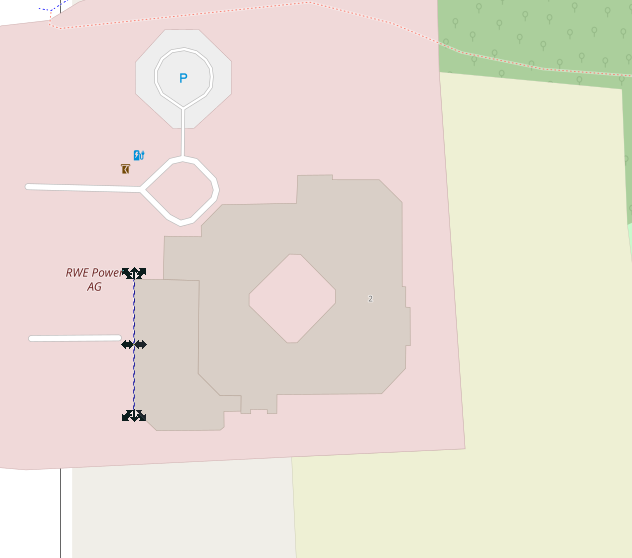
\includegraphics[width=0.5\textwidth]{Images/rwe.png}	
%	\end{subfigure}
%	\begin{subfigure}{0.5\textwidth}
		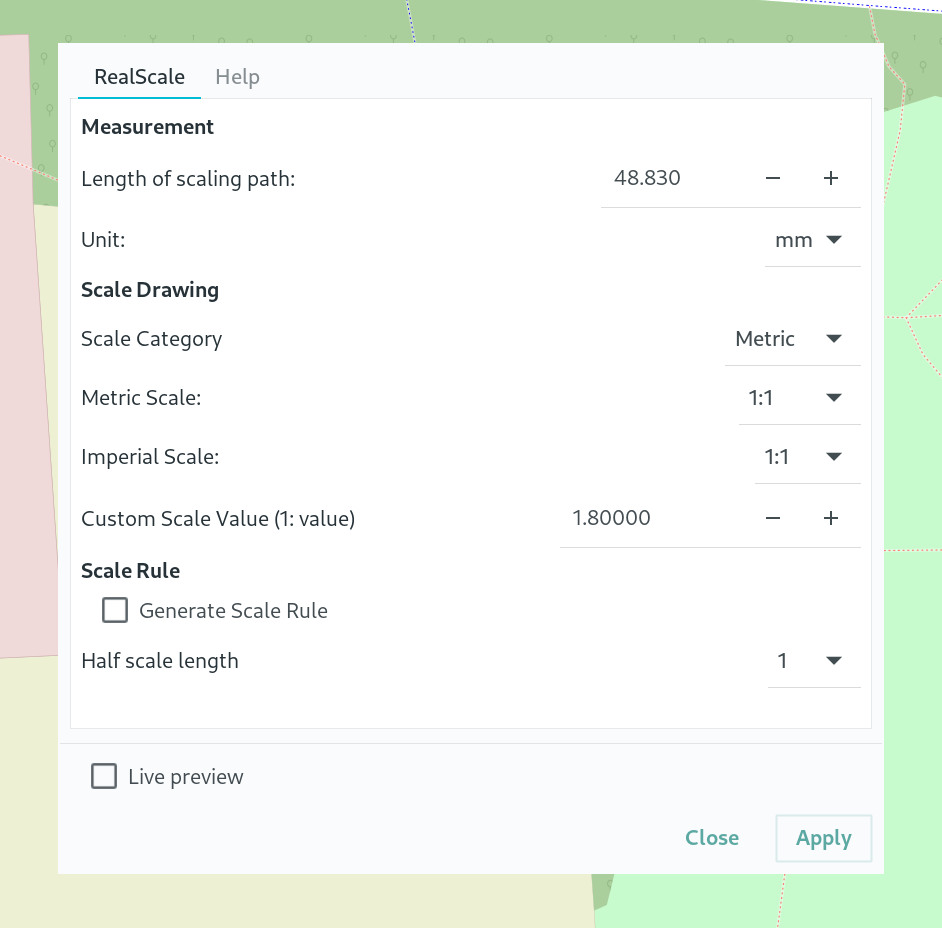
\includegraphics[width=0.5\textwidth]{Images/realscale.png}	
%	\end{subfigure}
	\caption{Skalierung}
	\label{fig:scaling_ausfuellen}
\end{figure}

Jetzt ist die Karte sklaliert! 1 mm in Inkscape entspricht einem Meter der Karte. Natürlich kann die Karte auch per Hand, ohne RealScale, skaliert werden.



\textbf{WICHTIG}: Darauf achten, dass bei der Erstellung von Objekten, deren Verschiebung oder Größenänderung \textbf{IMMER} \texttt{mm} als Einheit in der Menüleiste ausgewählt ist. Sonst wird der Maßstab von Elementen nicht eingehalten! (s. Abbildung \ref{fig:mm})

Die Größe von Elementen kann jetzt maßstabsgetreu angepasst werden. Für ein SG50-Zelt mit den Ausmaßen 5.64x10 Meter kann für \texttt{W} und \texttt{H} (lilane Pfeile in Abbildung \ref{fig:mm}, 5.64 und 10 eingetragen werden. 

\clearpage

\begin{figure}[!h]
	\centering
	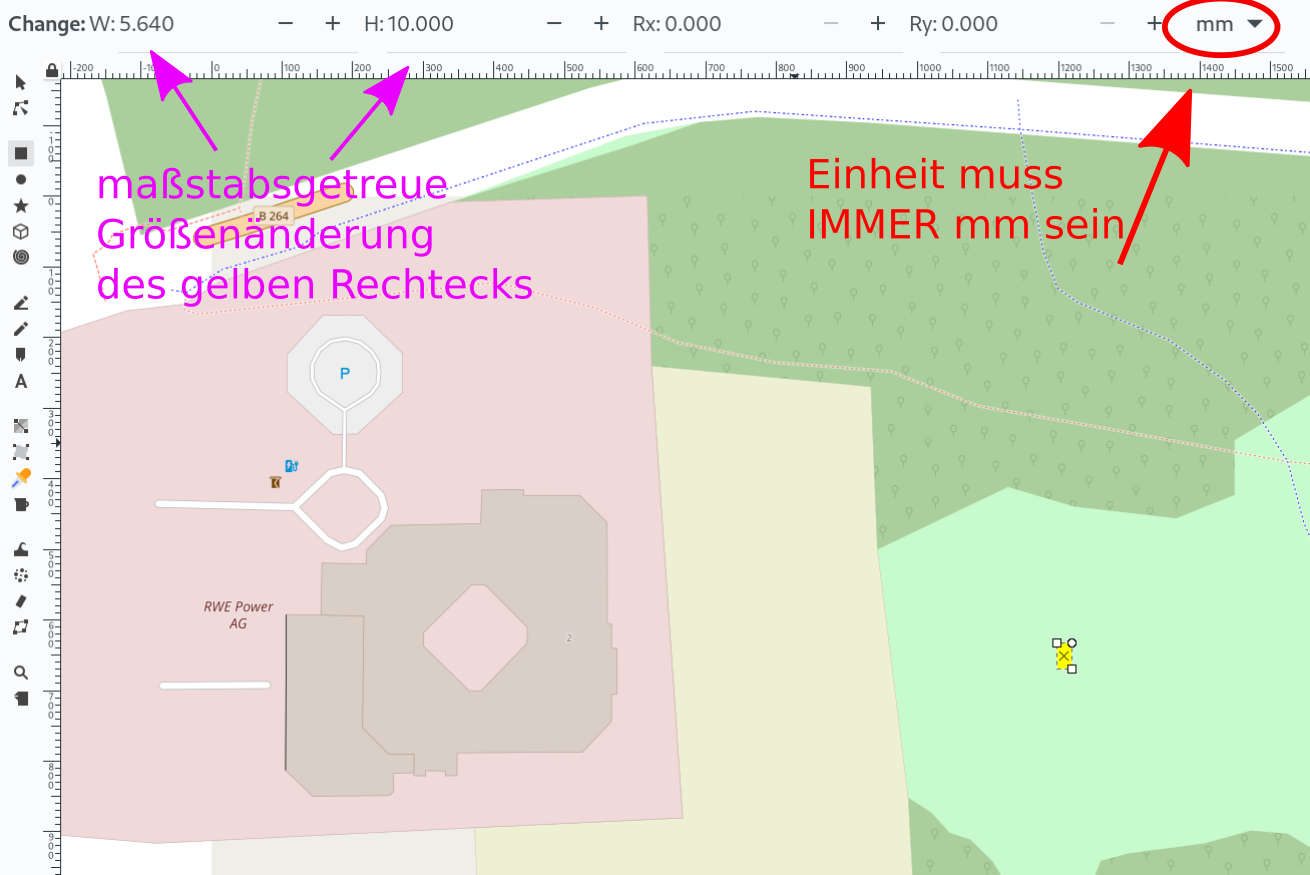
\includegraphics[width=0.7\textwidth]{Images/mm.png}
	\caption{Maßstabsgetreue Größenänderung}
	\label{fig:mm}
\end{figure}


\section{Hinzufügen von Elementen zum Aufbauplan}

In der Aufbauplanvorlage befinden sich bereits unterschiedliche Infrastrukturelemente, wie unterschiedliche Zelttypen (SG30, SG50, Zirkuszelte) und Sanitäranlagen. Es bietet sich an diese auf unterschiedlichen Ebenen zu sortieren.

Die Kennzeichnung der Rettungswege und der hygienischen Einbahnstraßen sollte auf jeden Fall auf unterschiedlichen Ebenen geschehen, so können diese einfach ein- und ausgeblendet werden, je nachdem, ob sie auf dem aktuellem Plan eingezeichnet werden sollen. In der Aufbauplanvorlage befinden sie sich auf den Ebenen \texttt{rettungswege} bzw. \texttt{hygiene}.

\section{Export}

Für den Export von Plänen kann eine neue Ebene \flqq{}Export\frqq{} angelegt werden. Diese enthält einzig ein Rechteck der Größe, des zu exportierenden Abschnittes. Die \flqq{}Opacity\frqq{} (Sichtbarkeit) der Ebene kann runtergeregelt werden, sodass der Aufbauplan noch sichtbar ist (s. Abbildung \ref{fig:exportlayer}).


	
\clearpage

\begin{figure}[!h]
	\centering
	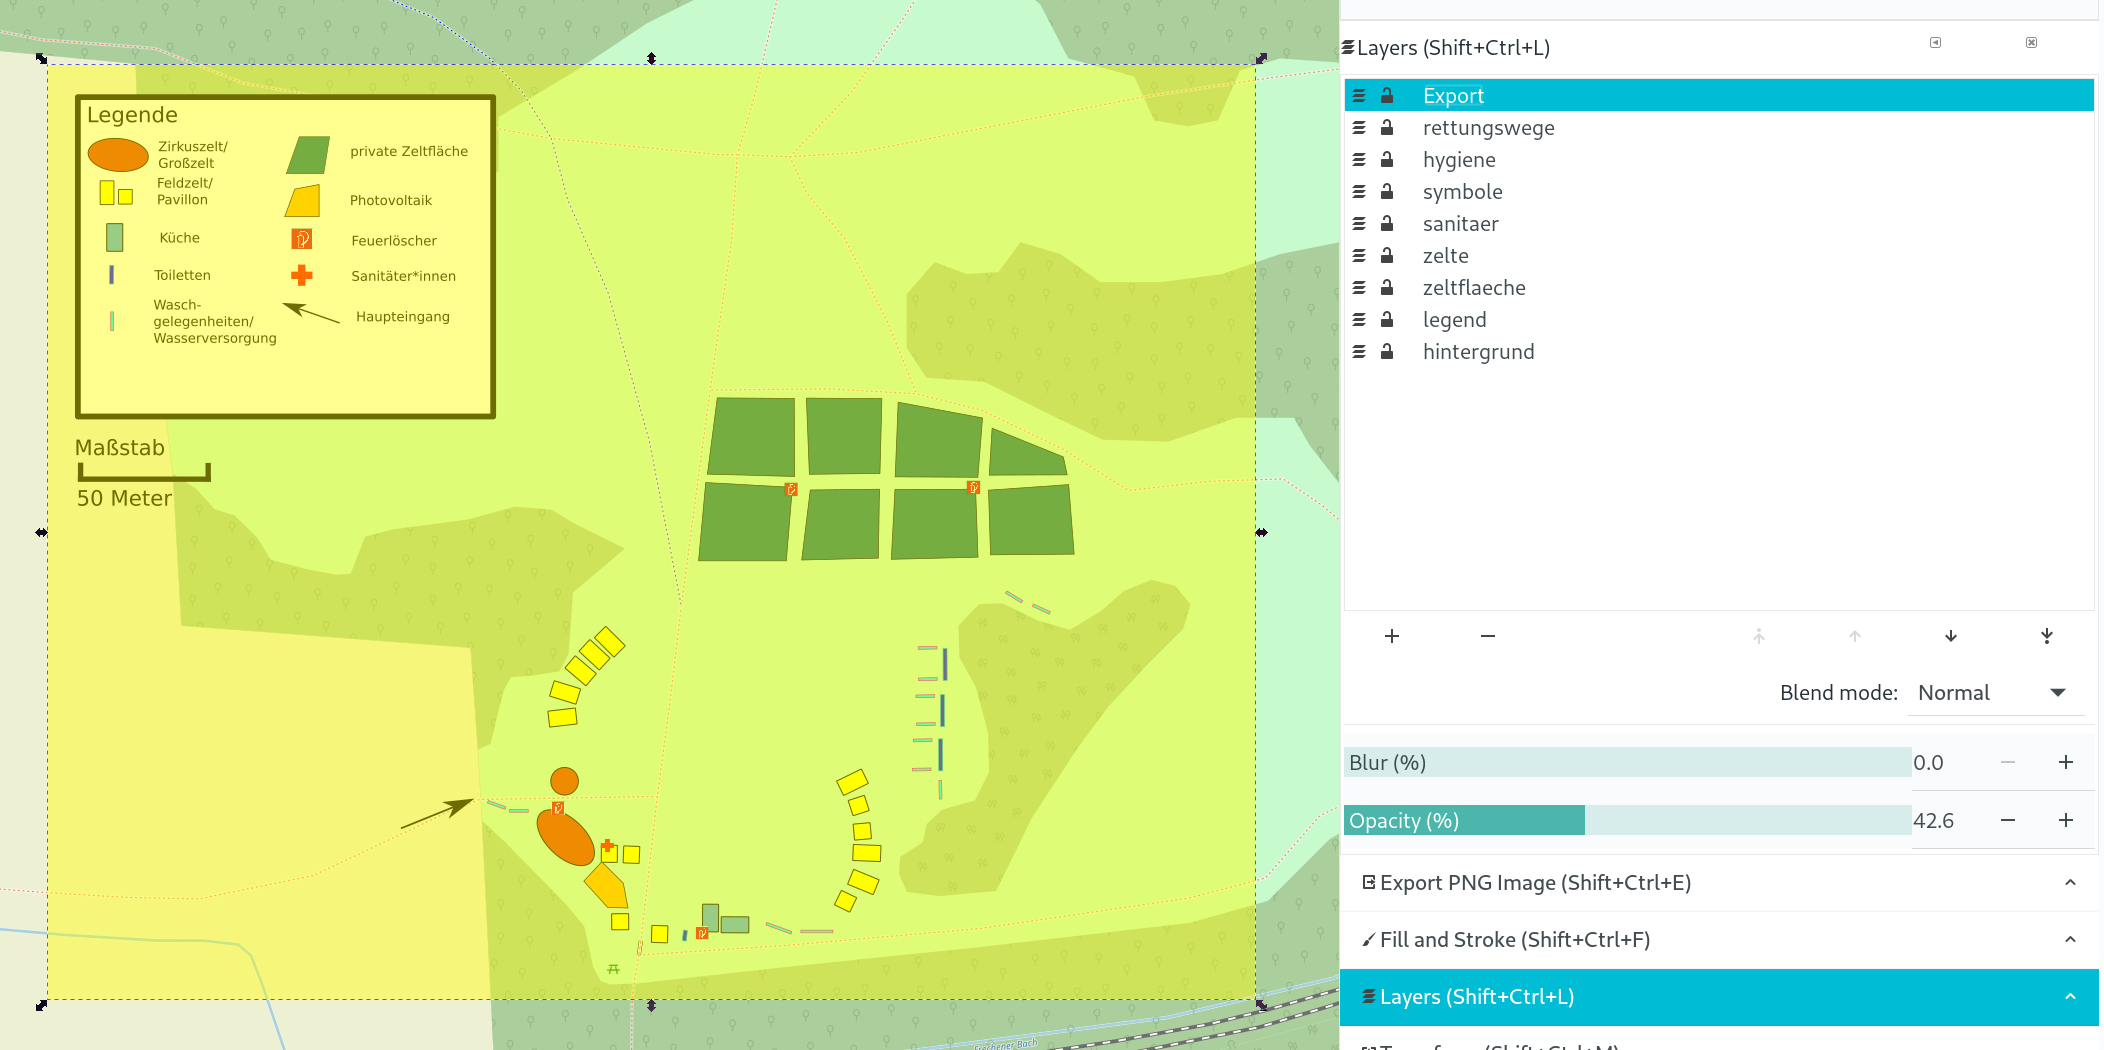
\includegraphics[width=\textwidth]{Images/export.png}
	\caption{Exportebene}
	\label{fig:exportlayer}
\end{figure}


Dieses Exportrechteck kann jetzt ausgewählt werden und die Exportebene mit Klick auf die drei Ebenen im Layers-Fenster unsichtbar machen. Die Größe des Exportrechtecks bleibt gestrichelt. Nun mit \texttt{Shift+Ctrl+E} das PNG-Export-Fenster öffnen.

Sicherstellen, dass \texttt{Selection} ausgewählt ist und \flqq{}Exportieren\frqq{} drücken (s. Abbildung \ref{fig:export2}).

\begin{figure}[!h]
	\centering
	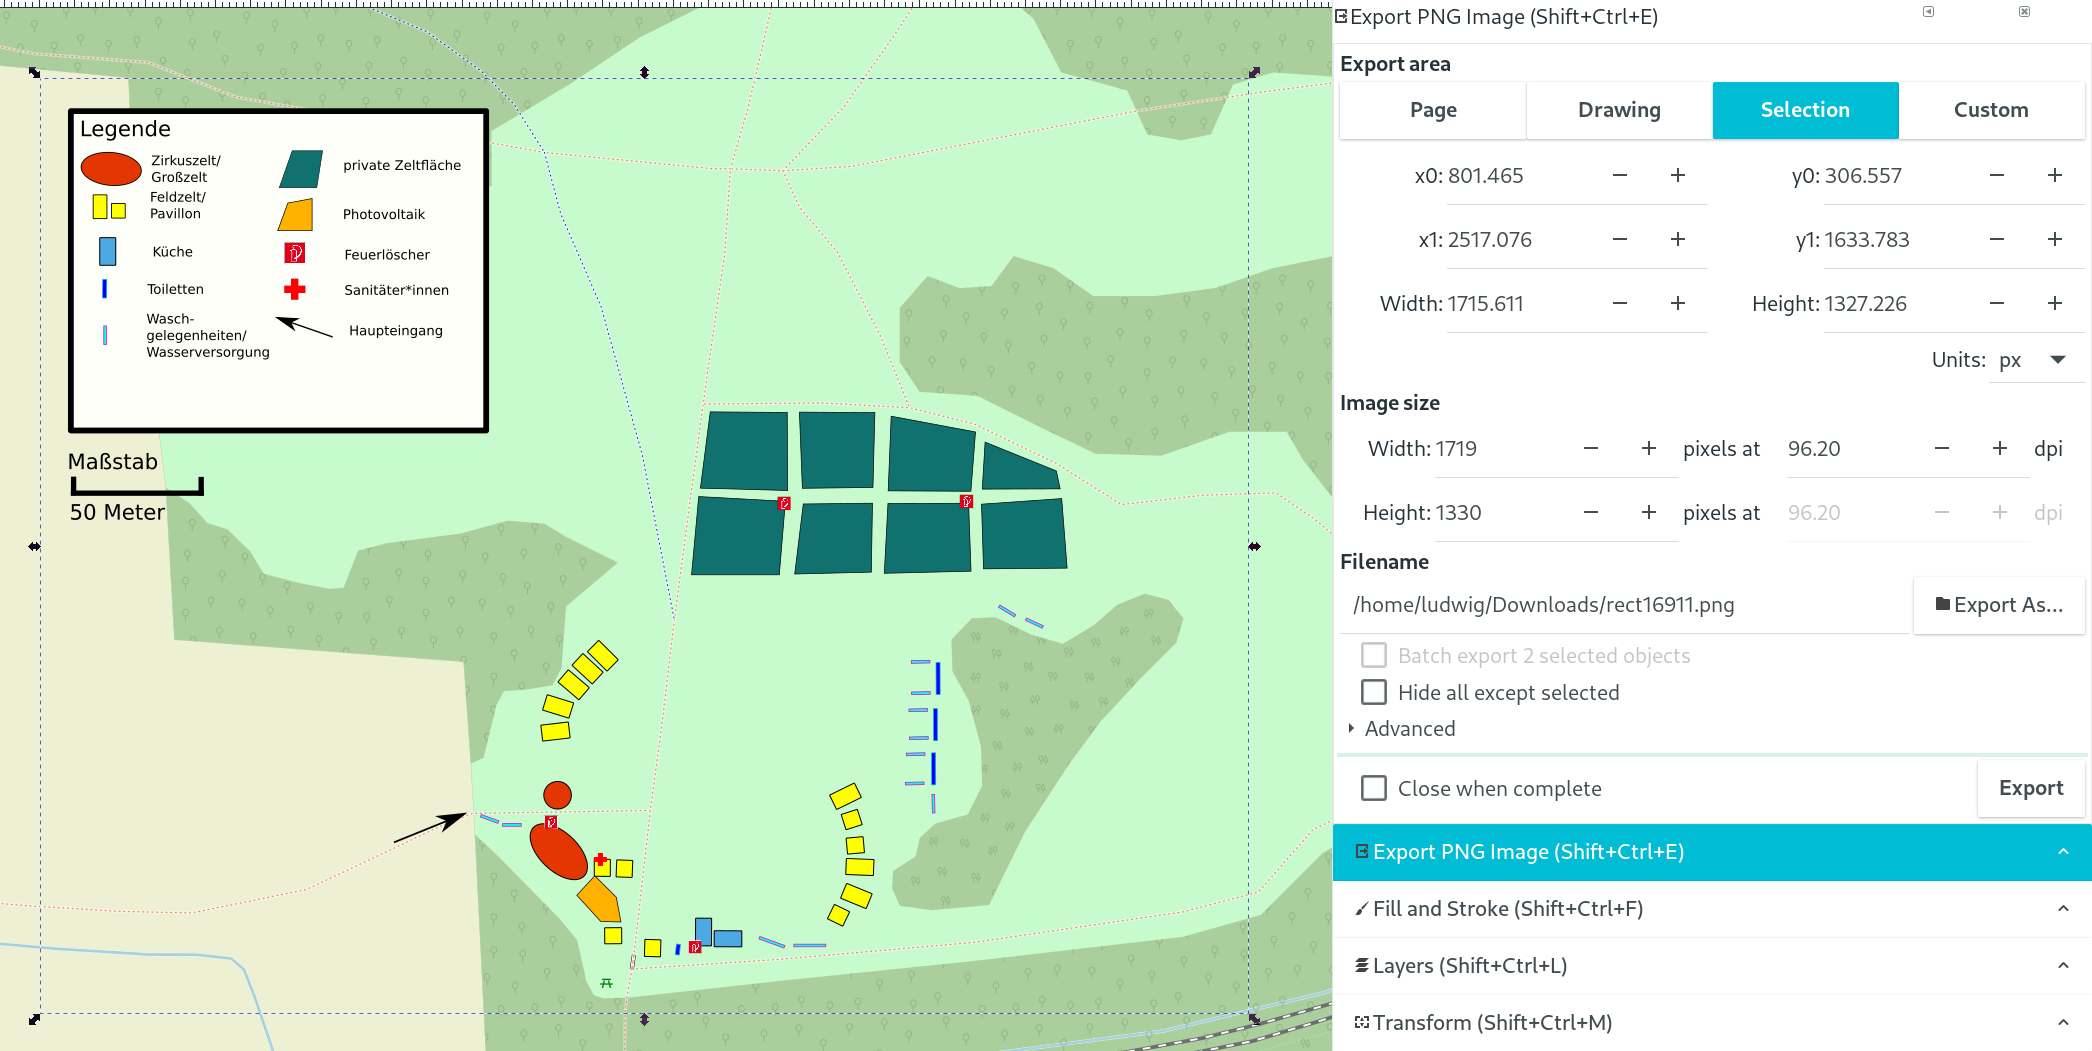
\includegraphics[width=\textwidth]{Images/export2.png}
	\caption{Export}
	\label{fig:export2}
\end{figure}

Tadaa. Der Aufbauplan ist fertig! Für den Rettungs- und Evakuierungsplan oder den Hygieneplan nur die entsprechenden Ebenen einblenden und wieder exportieren.

\end{document}
